\documentclass{article}
\def \Bx{x}
\def \x{{\mathbf x}}
\def \y{{\mathbf y}}
\def \Bf{{\mathbf f}}
\def \BM{{\mathbf M}}
\def \Bm{{\mathbf m}}
%\def \r{{\mathbf r}} !! sovrascrive \r{A}
\def \w{{\mathbf w}}
\def \z{{\mathbf z}}
\def \o{{\mathbf o}}
\def \i{{\mathbf i}}
\def \j{{\mathbf j}}
\def \g{{\mathbf g}}
\def \M{{\mathbf M}}
\def \calX{{\cal X}}
\def \calS{{\cal S}}
\def \calT{{\cal T}}
\def \calG{{\cal G}}
\def \calH{{\cal H}}
\def \calF{{\cal F}}
\def \calY{{\cal Y}}
\def \calZ{{\cal Z}}
\def \calD{{\cal D}}
\def \calR{{\cal R}}
\def \calL{{\cal L}}
\def \calC{{\cal C}}
\def \mcalA{{\mathcal A}}
\def \mcalV{{\mathcal V}}
\def \mcalE{{\mathcal E}}
\def \mcalL{{\mathcal L}}
\def \Rgen{R_{gen}}
\def \Remp{R_{emp}}
\def \be{\begin{equation}}
\def \ee{\end{equation}}
\newcommand{\ps}[1]{\left\langle #1 \right\rangle}
\newcommand{\pp}[2]{\mathbb{P}_{#1}\left[#2 \right]}
\newcommand{\RR}{\mathbb{R}}
\newcommand{\Rmd}{R_{\SSS \mbox{\rm emp}}^\delta}
\newcommand{\Ez}[1]{\mathbb{E}_z\left[#1 \right]}
\newcommand{\Er}[1]{\mathbb{E}_{\mathbf{r}}\left[#1 \right]}
\newcommand{\EDz}[2]{\mathbb{E}_{{\cal D}_\ell,#1}\left[ #2 \right]}
\newcommand{\EDsz}[2]{\mathbb{E}_{{\cal D}_\ell^\sigma,#1}\left[ #2 \right]}
\newcommand{\ED}[1]{\mathbb{E}_{\calD_\ell}\left[#1 \right]}
\newtheorem{theorem}{Theorem}[section]
\newtheorem{example}{Example}[section]
\newtheorem{defn}{Definition}[section]
\newtheorem{prop}{Proposition}[section]
\newtheorem{lemma}{Lemma}[section]
\newtheorem{definition}{Definition}[section]
\newtheorem{corollary}{Corollary}[section]
\newtheorem{prob}{Problem}[section]
\newcommand{\real}{{\rm I\!R}}
\newcommand{\nat}{{\rm I\!N}}
\newcommand{\al}{\alpha}
\newcommand{\bt}{\beta}
\newcommand{\AL}{\mbox{\boldmath $\alpha$}}
\newcommand{\THETA}{\mbox{\boldmath $\theta$}}
\newcommand{\XI}{\mbox{{\footnotesize \boldmath $\xi$}}}
\newcommand{\SSS}{\scriptscriptstyle}
\def\boldf#1{\mbox{\boldmath{$#1$}}}
\newcommand{\chem}[1]{\texttt{#1}}
\newcommand{\mchem}[1]{\mathrm{#1}}
\def \angstrom{\AA}
\def \argmax{\mbox{argmax}}
\def\minimize{\operatornamewithlimits{minimize}}

\usepackage{amsmath}
\usepackage{cancel}
\usepackage{bbm}
\usepackage{graphicx}
\usepackage{color}


\newcommand{\todo}[1]{\textcolor{blue}{{\bf [TODO]} #1}}

\begin{document}

\title{Constrained Adversarial Networks}
\author{Andrea Passerini}

\maketitle

We would like to incorporate constraints to GANs in an implicit way,
by an additional teacher penalizing outputs which do not satisfy the
constraints.

\todo{Why do we want to incorporate the constraints? }

The idea is to combine two recent works: Boundary-seeking
GANs~\cite{bgan} for dealing with discrete outputs, and posterior
regularization~\cite{Ganchev2010} for implicitly enforcing logic constraints to
deep nets~\cite{logicdeep}.

\section{Boundary-seeking GANs}

The idea is to train the generator to match a target distribution,
which at the limit of the perfect discriminator matches the data
distribution.

Given the (unknown) data distribution $p_{data}(\x)$, the generator
distribution $p_g(\x)$ and the discriminator $D(\x)$, we have that for
the perfect discriminator it holds (regardless of how $p_g(\x)$
matches $p_{data}(\x)$):
$$
D^*(\x) = \frac{p_{data}(\x)}{p_{data}(\x)+p_g(\x)}
$$
from which we can derive a formula for the data distribution:
$$
p_{data}(\x) = \frac{D^*(\x)}{1-D^*(\x)}p_g(\x)
$$
Given an imperfect discriminator $D(\x)$, we can approximate the
data distribution as:
$$
\tilde{p}_{data}(\x) = \frac{1}{Z} \frac{D(\x)}{1-D(\x)}p_g(\x)
$$
with
$$
Z = \sum_x \frac{D(\x)}{1-D(\x)}p_g(\x)
$$
When considering the noise $\z$ in input to the generator, it is
convenient to focus on joint distributions ($data$ dropped for
simplicity):
$$
p_g(\x,\z)=g(\x|\z)p(\z)
$$
and
$$
\tilde{p}(\x,\z) = \frac{1}{Z_{|\z}} \frac{D(\x)}{1-D(\x)}g(\x|\z)p(\z)
$$
where $g(\x|\z)$ is the generator's output (before discretization) for
input $\z$ and $Z_{|\z}=\sum_{\x} \frac{D(\x)}{1-D(\x)}g(\x|\z)$. Learning
the generator now amounts at minimizing its Kullback-Leibler divergence
to the estimated data distribution:
$$
\min_g D_{KL}( \tilde{p}(\x,\z) || p_g(\x,\z))
$$
See Appendix~\ref{app:dkl_gradient} for a detailed derivation of the gradient.

\section{Harnessing Deep Neural Networks with Logic Rules}

The idea is to jointly train two models: the student ($p(\y|\x)$)
minimizes a combination of a loss function on supervised data and a
loss function on predictions made by the teacher; the teacher
($q(\y|\x)$) minimizes the KL divergence to the student model and the
number of rule violations.

\noindent The student minimization problem is:
\begin{align*}
  \min_\theta \sum_{(\x,\y) \in \calD} \gamma \ell(\y,p_\theta(\y|\x)) + (1-\gamma) \ell(q(\y|\x),p_\theta(\y|\x))
\end{align*}
The teacher minimization problem is:
\begin{align*}
  \min_q & \quad D_{KL}(q(\y|\x)||p_\theta(\y|\x)) + C \sum_{l,g_l} \xi_{l,g_l}  \\
  s.t. &  \quad \lambda_l(1 - E_q[r_{l,g_l}(\y,\x)]) \le \xi_{l,g_l} \quad \forall l, \forall g_l 
\end{align*}
Here $l$ ranges over the set of rules, $g_l$ over the set of rule
groundings on $(\x,\y)$, $r_{l,g_l}(\y,\x)$ computes the soft rule
using e.g. the Lukasiewicz t-norm, and $\lambda_l$ is the strength of
rule $l$. The problem has a closed-form solution given by:
$$
q(\y|\x) \propto p_\theta(\y|\x) \exp{\left[-\sum_{l,g_l} C \lambda_l (1 - r_{l,g_l}(\y,\x))\right]}
$$
The complexity of computing the normalization factor depends on the
rules. In the worst case, one needs to resort to approximation
strategies (e.g. Gibbs sampling). As a very first approximation, one
could employ an importance sampling strategy similar to the one
used in BGANs, i.e. sample according to $p_\theta(\y|\x)$ and reweight
by
$\exp{\left[-\sum_{l,g_l} C \lambda_l (1 - r_{l,g_l}(\y,\x))\right]}$.


\section{Possible directions}
The first two directions consist in modifying the BGAN framework by
providing either the discriminator or the generator with a signal on
the satisfaction of the constraints $\Psi(\mathbf{x})$. An alternative
direction is to introduce a third network (the teacher $T$) that is
trained to ``improve'' the objects generated by $G$ by modifying them
in order to satisfy the constraints. The generator is trained not only
to fool the discriminator, but also to approximate the teacher's
distribution (this closely resembles the approach presented
in~\cite{logicdeep}). \todo{Add the reinforcement learning-based direction}.

\subsection{Constraint-regularized discriminator}
\begin{align*}
  l_G &= E[D(G(\mathbf{z}))]_{\mathbf{z} \sim P_\mathbf{z}} \\
  l_D &= E[D(\mathbf{x},\Psi(\mathbf{x}))]_{\mathbf{x} \sim P_{\mathbf{x}}} + E[1 - D(G(\mathbf{z}),\Psi(G(\mathbf{z})))]_{\mathbf{z} \sim P_{\mathbf{z}}}
\end{align*}
The discriminator is provided with both an object $\mathbf{x}$ and a
signal on the satisfaction of the constraints $\Psi(\mathbf{x})$.  By
making the discriminator aware of $\Psi$, the generator should be
pushed to generate objects which satisfy the constraints \textcolor{red}{(as long as
  those constraints are also satisfied in the training data)}.

Since $l_G$ is constraint-agnostic, this approach can be used even
with constraints that are not differentiable and with constraints that
cannot be written (or are difficult to write) in closed form.

\subsection{Constraint-regularized generator}
\begin{align*}
  l_G &= E[D(G(\mathbf{z}))]_{\mathbf{z} \sim P_\mathbf{z}} + \lambda E[\Psi(G(\mathbf{z}))]_{\mathbf{z} \sim P_{\mathbf{z}}} \\
  l_D &= E[D(\mathbf{x})]_{\mathbf{x} \sim P_{\mathbf{x}}} + E[1 - D(G(\mathbf{z}))]_{\mathbf{z} \sim P_{\mathbf{z}}}
\end{align*}
Another approach is to incorporate the signal on the constraint
satisfaction $\Psi$ in the generator loss $l_G$ as a regularization
term with weight $\lambda$. \todo{Pros and cons?}


\subsection{Teacher-based training}
\begin{align*}
  l_G &= E[D(G(\mathbf{z}))]_{\mathbf{z} \sim P_\mathbf{z}} + \lambda E[D_{KL}(T(G(\mathbf{z})),G(\mathbf{z})]_{\mathbf{z} \sim P_{\mathbf{z}}} \\
  l_D &= E[D(\mathbf{x})]_{\mathbf{x} \sim P_{\mathbf{x}}} + E[1 - D(G(\mathbf{z}))]_{\mathbf{z} \sim P_{\mathbf{z}}}\\
  l_T &= E[\Psi(T(G(\mathbf{z})))]_{\mathbf{z} \sim P_{\mathbf{z}}}
\end{align*}  

  \bibliographystyle{plain} \bibliography{notes}

\appendix

\section{Gradient of $D_{KL}(\tilde{p}(\x,\z) || p_g(\x,\z))$}
\label{app:dkl_gradient}

Let $\theta$ be the parameters of $g(\x|\z)$. Let's assume
$\tilde{p}(\x,\z)$ is constant with respect to $\theta$, i.e. we use
the $\theta$ from the previous iteration and do not propagate their gradient inside $\tilde{p}$.

\begin{align*}
\nabla_\theta D_{KL}( \tilde{p}(\x,\z) || p_g(\x,\z))) & =  \nabla_\theta \sum_\z \sum_\x \tilde{p}(\x,\z) \log{\frac{\tilde{p}(\x,\z)}{p_g(\x,\z)}} \\
& = - \sum_\z \sum_\x \frac{1}{Z_{|\z}}\frac{D(\x)}{1-D(\x)}g(\x|\z)p(\z) \nabla_\theta\log{g(\x|\z)} \\
& = - E\left[\sum_\x \frac{1}{Z_{|\z}}\frac{D(\x)}{1-D(\x)}g(\x|\z) \nabla_\theta\log{g(\x|\z)}\right]_{\z \sim p(\z)}\\
& \approx - E\left[\sum_m \frac{1}{M}\frac{1}{Z_{|\z}}\frac{D(\x^{(m)})}{1-D(\x^{(m)})}\nabla_\theta\log{g(\x^{(m)}|\z)}\right]_{\z \sim p(\z)}
\end{align*}
where we approximated the gradient using $M$ samples
$\x^{(m)} \sim g(\x|\z)$ for each $\z$ ($g(\x|\z)$ computes a
probability for each component of $\x$, e.g. sigmoid for binary
variables, and selecting $\x^{(m)}$ amounts at sampling the discrete
values from that probability). The samples can also be used to
approximate $Z_{|\z}$ as:
$$
Z_{|\z} = \sum_{\x} \frac{D(\x)}{1-D(\x)}g(\x|\z) \approx \sum_m  \frac{1}{M}\frac{D(\x^{(m)})}{1-D(\x^{(m)})}
$$

\noindent Alternatively, one can use $D_{KL}(p_g(\x,\z) || \tilde{p}(\x,\z))$:

\begin{align*}
\nabla_\theta D_{KL}( p_g(\x,\z) || \tilde{p}(\x,\z)) & =  \nabla_\theta \sum_\z \sum_\x g(\x|\z)p(\z) \log{\frac{p_g(\x,\z)}{\tilde{p}(\x,\z)}} \\
& =  \sum_\z \sum_\x p(\z) \left[ \nabla_\theta g(\x|\z)  \log{\frac{p_g(\x,\z)}{\tilde{p}(\x,\z)}} + g(\x|\z)  \nabla_\theta \log{g(\x|\z)} \right] \\
& = \sum_\z \sum_\x p(\z) g(\x|\z) \nabla_\theta \log{g(\x|\z)} \left[ \log{\frac{\cancel{g(\x|\z)}\cancel{p(\z)}}{\frac{1}{Z_{|\z}}\frac{D(\x)}{1-D(\x)}\cancel{g(\x|\z)}\cancel{p(\z)}}} + 1 \right] \\
& = \sum_\z \sum_\x p(\z) g(\x|\z) \nabla_\theta \log{g(\x|\z)} \left[\log{Z_{|\z}} - \log{\frac{D(\x)}{1-D(\x)}} + 1 \right]
\end{align*}
where we used the fact that $\nabla_\theta g(\x|\z) = g(\x|\z) \nabla_\theta  \log{g(\x|\z)}$

\section{$\nabla_\theta\log{g(\x^{(m)}|\z)}$ for binary variables}

Note that in practice, in~\cite{bgan}
$\nabla_\theta\log{g(\x^{(m)}|\z)}$ for binary variables is
approximated as:

\begin{align*}
\nabla_\theta\log{g(\x^{(m)}|\z)} & = \nabla_\theta \sum_{i=1}^{|\x^{(m)}|} \mathbbm{1}_{[x_i^{(m)} = 1]} \log{g_i(\x^{(m)}|\z)} + \mathbbm{1}_{[x_i^{(m)} = 0]} \log{(1 - g_i(\x^{(m)}|\z))} \\
& = \nabla_\theta \sum_{i=1}^{|\x^{(m)}|} \mathbbm{1}_{[x_i^{(m)} = 1]} \log{\sigma(h_i(\x^{(m)}|\z))} + \mathbbm{1}_{[x_i^{(m)} = 0]} \log{(1 - \sigma(h_i(\x^{(m)}|\z)))} \\
& =  \nabla_\theta \sum_{i=1}^{|\x^{(m)}|} \mathbbm{1}_{[x_i^{(m)} = 1]} \log{\frac{1}{1+\exp{-h_i(\x^{(m)}|\z)}}}+ \mathbbm{1}_{[x_i^{(m)} = 0]} \log{\frac{\exp{-h_i(\x^{(m)}|\z)}}{1+\exp{-h_i(\x^{(m)}|\z)}}} \\                                
& =  - \nabla_\theta \sum_{i=1}^{|\x^{(m)}|}\log{(1+\exp{-h_i(\x^{(m)}|\z)})} + \mathbbm{1}_{[x_i^{(m)} = 0]}h_i(\x^{(m)}|\z) \\
& \approx  - \nabla_\theta \sum_{i=1}^{|\x^{(m)}|}\max{(0,-h_i(\x^{(m)}|\z))} + \mathbbm{1}_{[x_i^{(m)} = 0]}h_i(\x^{(m)}|\z) \\
\end{align*}
where we used the approximation $\log{(1+\exp{-x})} \approx \max{(0,-x)}$, see Figure~\ref{fig:approx}.

\begin{figure}
  \centering
  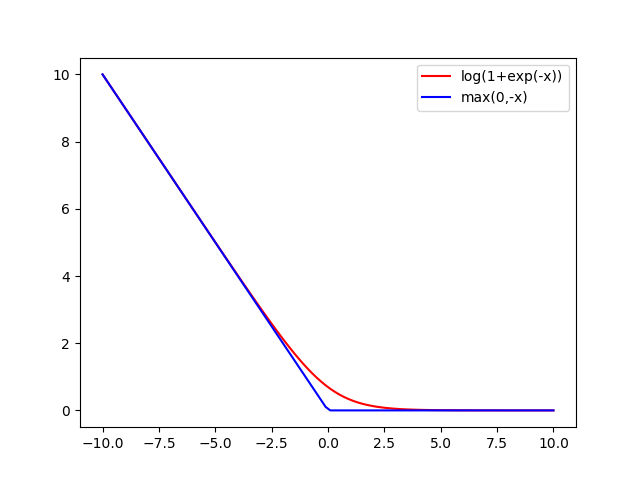
\includegraphics[width=.7\textwidth]{Figures/approx}
  \caption{\label{fig:approx}Approximated log gradient}
\end{figure}

\section{$\nabla_\theta\log{g(\x^{(m)}|\z)}$ for multinomial variables}



\begin{align*}
\nabla_\theta\log{g(\x^{(m)}|\z)} & = \sum_{i=1}^{|\x^{(m)}|} \sum_{j=1}^c \mathbbm{1}_{[x_i^{(m)} = j]} \nabla_\theta \log{ \frac{\exp{h_{i,j}(\x^{(m)}|\z)}}{\sum_{j' = 1}^c \exp{h_{i,j'}(\x^{(m)}|\z)}}} \\
  & = \sum_{i=1}^{|\x^{(m)}|} \sum_{j=1}^c \mathbbm{1}_{[x_i^{(m)} = j]} \left( \nabla_\theta h_{i,j}(\x^{(m)}|\z) -  \nabla_\theta \log{\sum_{j' = 1}^c \exp{h_{i,j'}(\x^{(m)}|\z)}}\right) \\
  & =  \sum_{i=1}^{|\x^{(m)}|} \sum_{j=1}^c \mathbbm{1}_{[x_i^{(m)} = j]} \left( \nabla_\theta h_{i,j}(\x^{(m)}|\z) - \frac{\sum_{j' = 1}^c \exp{h_{i,j'}(\x^{(m)}|\z)}\nabla_\theta h_{i,j'}(\x^{(m)}|\z)}{\sum_{j' = 1}^c \exp{h_{i,j'}(\x^{(m)}|\z)}} \right)
\end{align*}

\noindent where $c$ is the number of possible values of each
multinomial variable, $h_{i,j}(\x^{(m)}|\z)$ is the output of the
$j^{th}$ channel for the $i^{th}$ variable, corresponding to the
unormalized probability of outcome $j$ for that variable.

\end{document}
